\documentclass{article}
% main document, called main.tex
\usepackage{newtxtext,newtxmath}
% Depending on your LaTeX fonts installation, you might get better results with one of these:
%\usepackage{mathptmx}
%\usepackage{txfonts}

% Use vector fonts, so it zooms properly in on-screen viewing software
% Don't change these lines unless you know what you are doing
\usepackage[T1]{fontenc}
\usepackage{ae,aecompl}
\usepackage{graphicx}	% Including figure files
\usepackage{amsmath}	% Advanced maths commands
\usepackage{amssymb}	% Extra maths symbols
\usepackage{tikz}
\DeclareMathAlphabet{\mathcal}{OMS}{cmsy}{m}{n}
\usetikzlibrary{bayesnet}
\usetikzlibrary{external}
\tikzexternalize % activate!
\tikzset{external/force remake}
\begin{document}
	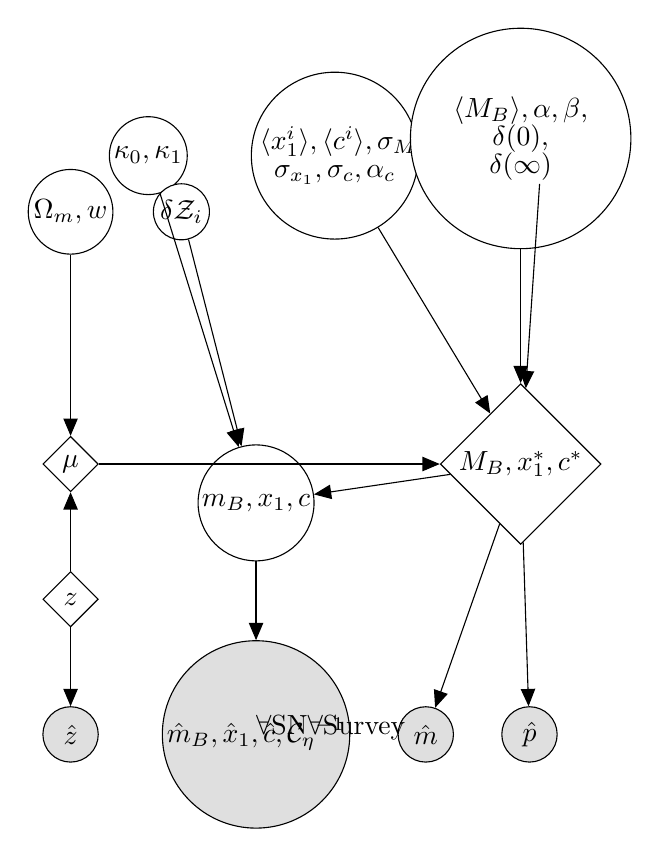
\begin{tikzpicture}
	% Obs nodes
	\node[obs]  (obssum) {$\hat{m}_B, \hat{x}_1, \hat{c}, \mathcal{C_\eta}^{-1}$};
	\node[obs, left=0.8cm of obssum]  (zobs) {$\hat{z}$};
	\node[obs, right=0.6cm of obssum]  (mobs) {$\hat{m}$};
	\node[obs, right=0.6cm of mobs]  (pobs) {$\hat{p}$};
	% Latent nodes
	\node[latent, above=of obssum] (sum) {$m_B, x_1, c$};
	\node[det, above=of zobs] (z) {$z$};	
	\node[det, above=of z] (mu) {$\mu$};
	\node[det, right=4.33cm of mu] (MBobs) {$M_B, x_1^*, c^*$};
	% Survey nodes
	\node[latent, above=of sum, yshift=1.6cm, xshift=1cm, text width=1.9cm, align=center] (pop1) {$\langle x_1^i \rangle, \langle c^i \rangle,\sigma_{M_B}, $\\$ \sigma_{x_1}, \sigma_c, \alpha_c$ };
	\node[latent, right=1.2cm of pop1, align=center] (sf) {$\delta S$};
	\node[latent, left=0.8cm of pop1, align=center] (kappa) {$\kappa_0, \kappa_1$};
	% Global nodes
	\node[latent, above=2.3cm of mu]  (cosmo) {$\Omega_m, w$};
	\node[latent, above=1.7cm of MBobs, text width=2.5cm, align=center]  (ab) {$\langle M_B \rangle, \alpha, \beta$, $\delta(0)$, \\$\delta(\infty)$};
	\node[latent, right=0.5cm of cosmo, align=center]  (dz) {$\delta \mathcal{Z}_i$};
	% Connect the nodes
	\edge {sum} {obssum};
	\edge {z} {zobs};
	\edge {z,cosmo} {mu};
	\edge {mu, pop1, ab, sf} {MBobs};	
	\edge {MBobs} {pobs, mobs};
	\edge {dz, kappa, MBobs} {sum};
	% Plates
	\plated[thick] {sn} {(obssum)(zobs)(mobs)(pobs)(sum)(z)(mu)(MBobs)} {$\forall\ \rm{SN}$} ;
	\plated[thick] {survey} {(sn)(pop1)(kappa)(sf)} {\\$\forall\ \rm{Survey}$} ;
	\end{tikzpicture}
\end{document}